In this section, we present our measurement methodology along with the
metrics considered and discuss energy efficiency and power-performance
traces of the model system.

\subsection{Measurement methodology}
\label{subsec:4.1}

We  approach  the  assessment  of  the energy  footprint  and  overall
performance   of   \cosmoart   with  two   important  metrics:
\textit{time-to-solution} (TTS) and \textit{energy-to-solution} (ETS).
TTS refers to  the total wall clock time  of the application execution
time. ETS  is the amount of  energy spent to  achieve results.  Energy
consumption  is  assessed by  sampling  the  power during execution which is then averaged and multiplied  by the TTS to determine  ETS. Whenever  possible,  multiple production  runs  were
performed  to  illustrate the  reproducibility  of  the baseline,  and
quantify the  significant uncertainties  in the power  measurement, as
dictated by the available technology.

For all the experiments we also analyze the contribution of the MPI library to the energy consumption and how the use of the blocking versus polling message-passing policies can potentially render energy savings. Specifically, the OpenMPI 1.6.5 library installed in \tinto, features two operation modes, blocking and modes, which can be selected before \cosmoart is launched. In the polling configuration (the detault mode) ``MPI'' continually polls
the netwrok interface to check for the completion of an event (e.g. send or receive).
This usually yields low latency but high CPU utilization. Thus, can one expcet that this mode attanins the best performance, possibley at the cost a higher energy usage. In the blocking
mode, the CPU is yield to other processes/threads if there are no incoming messages.


\subsection{Time-power-energy analysis of \cosmoart}
\label{subsec:4.2}

\begin{figure}[htbf]
  \begin{center}
    \includegraphics[width=0.48\textwidth]{Figs/NRJ_benchmark_Monch.eps}
    \caption{\monch: Isola E1 Rack 2 Total Power.}
    \label{fig:1}
  \end{center}
\end{figure}

\begin{figure}[htbf]
  \begin{center}
    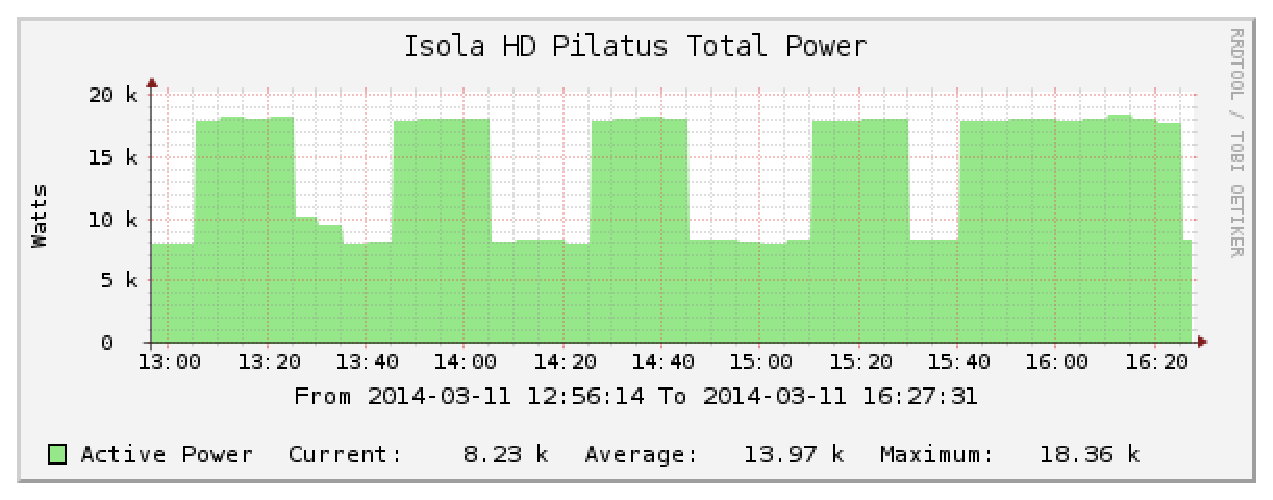
\includegraphics[width=0.48\textwidth]{Figs/NRJ_benchmark_Pilatus.eps}
    \caption{\pilat: Isola HD Total Power.}
    \label{fig:2}
  \end{center}
\end{figure}

Figures~\ref{fig:1}   and   \ref{fig:2}   account   respectively   for
\monch's Isola E1 Rack  2 and \pilat' Isola HD total
power measurements for  1-day or 2-days simulations. On  the Intel Ivy
Bridge EP  based cluster (i.e.  \monch),  the 1-day simulation
was issued  only twice due  to usage restrictions. As  time resolution
was set to one update every  5 minutes for power sampling, the average
power consumption was computed by considering 6 values for each single
run.  On the Intel Xeon E5 based cluster (i.e.  \pilat), the
1-day simulation  was issued  four times and  a 2-days run  only once.
Similarly, the average power consumption was computed by considering 4
values  for  each  single  1-day  run  and 9  values  for  the  2-days
run. Corresponding results are gathered in Table~\ref{tab:3}.

\begin{table}[htbf]
  \begin{center}
    \caption{Average power consumption (W) of the platforms}
    \label{tab:3}
    \begin{tabular}{cccc}
      \hline\noalign{\smallskip}
      \textbf{\scriptsize{Xeon E5}} & \textbf{\scriptsize{Ivy Bridge}} & \textbf{\scriptsize{Xeon  E5645}} & \textbf{\scriptsize{Xeon  E5645}}\\
      & & \textbf{\scriptsize{(Polling)}} & \textbf{\scriptsize{(Blocking)}} \\
      \noalign{\smallskip}\hline\noalign{\smallskip}
      18035.0 & 12622.5 & 3713.6 & 3651.8 \\ 
      \noalign{\smallskip}\hline
    \end{tabular}
  \end{center}
\end{table}

In  Figure~\ref{fig:3}, we  compare both  TTS (right  Y-axis)  and ETS
(left  Y-axis)  metrics  on  both  platforms.  As  expected,  Xeon  E5
outperforms Ivy Bridge EP, being  roughly 1.3x faster.  The reason for
that is  two-fold: \emph{i}) it has  higher clock frequency  than Ivy Bridge
(2.6  GHz  against  2.2 GHz),  and  \emph{ii})  it  aims at  computing  speed
regardless to  energy consumption.  In our experiments,  Ivy Bridge EP
showed the best energy-to-solution, reducing the energy consumption of
Xeon E5 by approximately 7\,\%.

The TTS and ETS results for a full-day simulation on \tinto are shown in Figure~\ref{fig:4}.  As expected, the mean energy consumed by COSMO-ART when using the blocking MPI policy is about 2\,W less than that consumed by the polling mode. This is due to the blocking-waits performed by the CPU cores while using the blocking mode, in contrast of the polling-waits that take place when polling mode is used. From the point of view of the execution time, there is a slight reduction when the blocking MPI policy is leveraged. One can expect that the costs of the interruptions used in the blocking MPI policy can lead to an increase of the total execution time, however, applications with extensive computing may show better perforamnce with the blocking modes. This plays in favour for our results since the energy consumed is also less by just changing the behavior of the OpenMPI library from the polling to the blocking policy.



\begin{figure}[htbf]
  \includegraphics[width=0.5\textwidth]{Figs/Time_E2S_COSMO-ART-0.eps}
  \caption{Time-to-solution and energy-to-solution comparison between
    Xeon E5 and Ivy Bridge-EP architectures for a 24h simulation.}
  \label{fig:3}
\end{figure}

\begin{figure}[htbf]
  \includegraphics[width=0.5\textwidth]{Figs/Time_E2S_COSMO-ART-5.eps}
  \caption{Mean time-to-solution and energy-to-solution on
    \textsc{Tintorrum} for a 24h simulation using the polling and blocking MPI policies.}
  \label{fig:4}
\end{figure}

\subsection{Power-performance tracing on \tinto}
\label{subsec:4.3}

A full tracing experiment is conducted on \tinto in order to capture an overall power
profile at a much finer resolution. First we run \cosmoart for a full-day simulation
and analyze the power consumption. Second we correlate performance with
power traces of two 1-hor time frames during the day: mid-day (from 11h-12h) and
midnight (23h-24h). All the experiments were performed using 192 \cosmoart processes
mapping 12 processes in each of node.

For all the experiments we also analyze the contribution of the MPI library to the energy 
consumption and how the use of the blocking versus polling message-passing policies can 
potentially render energy savings. Specifically, the OpenMPI 1.6.5 library installed in \tinto, 
features two operation modes, blocking and modes, which can be selected before \cosmoart is 
launched. In the polling configuration (the detault mode) ``MPI'' continually polls
the netwrok interface to check for the completion of an event (e.g. send or receive).
This usually yields low latency but high CPU utilization. Thus, can one expcet that this mode attanins the best performance, possibley at the cost a higher energy usage. In the blocking
mode, the CPU is yield to other processes/threads if there are no incoming messages.

In order to obtain an initial overview of the power dissipation of the system model, we have 
obtained the power profiles using our \pmlib framework of a full-day simulation of \cosmoart 
leveraging the polling and blocking MPI policies, these results are depicted in the top/bottom 
plots of Figure~\ref{fig:9}, respectvely. o, captured with our PDUs. The first observation for 
the polling MPI policy is the quite plain power profile it generates. However, the first and 
last hours of the full-day simulation dissipate slightly less power than the mid-day hours. We 
relate these variations due to the chemical reactions and aerosols, computed by ART, that are 
taking place during the daylight hours but not during night. In this case peak power 
dissipation is about 3821\,W. Looking at the power profile using the blocking MPI policy, we 
can easily observe that the pattern is repeated favoring the reduction of power during 
nighttime hours in a more  noticeable way. The peak power dissipation in this mode is 3768\,W, 
which means a reduction of 50\,W in total or, in other words, 1,\% of reductuon in the peak 
power. Also, we observe power  drops in each hour simulated, basically related to periods in 
which the processes were performing blocking-waits instead of polling-waits, thus yielding the 
CPU to a low usage during this phases. Our final observation is the reduction in execution time 
when the blocking MPI policy is leveraged in contrast with the polling MPI. One can expect that 
the costs of the interruptions used in the blocking can lead to an increase of the total 
execution time, however, applications with extensive computing may show better perforamnce with 
the blocking mode. This plays in favour for our results since the energy consumed is also less 
by just changing the behavior of the OpenMPI library from the polling to the blocking policy.

To gain more insights about the power-performance behavior of \cosmoart, we also have conducted 
experiments that show power-performance traces of 1 hour simulation. We limited the simulation 
time to this bound since the pattern of the computation performed by \cosmoart is repeated each 
hour, also because the weight of a full-day simulation trace can not be easily handled using 
our machines and memory available (about 45\,GB per trace file). To soften the problem we 
shrink the simulations to 1 hour during mid-day (11h-12h) and midnight (23h-24h), in which 
\cosmoart perform different internal computations, as shown in Figure~\ref{fig:9}. At the same
time we also leverage the two stated MPI policies: polling and waiting modes.



\begin{figure*}[htbf]
  \centering
  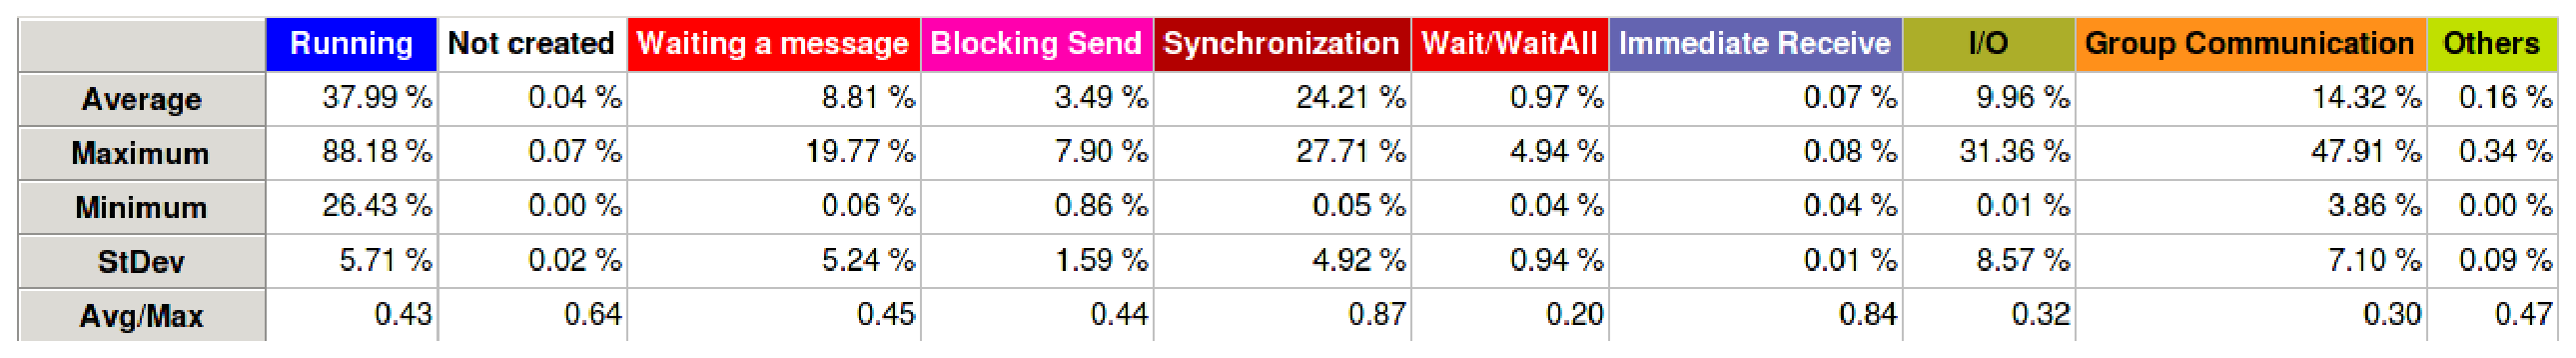
\includegraphics[width=0.78\textwidth]{Figs/23_24_blq1_stat1.eps}
  \caption{blabla}
  \label{fig:8}
\end{figure*}

\begin{figure*}[htbf]
  \centering
  \scalebox{0.5}{\input{Figs/24hour.pstex_t}}
  \caption{24 hours simulation trace using the MPI blocking mode on
    \textsc{Tintorrum}.}
  \label{fig:9}
\end{figure*}

\begin{figure*}[htbf]
  \centering
  \scriptsize
  % Simulation of 1 hour during midday (from 11h to 12h) leveraging the polling MPI policy\\
  % \scalebox{0.5}{\input{Figs/11_12_blq0_figure.pstex_t}}\\
  % Simulation of 1 hour during midday (from 11h to 12h) leveraging the blocking MPI policy\\
  % \scalebox{0.5}{\input{Figs/11_12_blq1_figure.pstex_t}}\\
  Simulation of 1 hour during midnight (from 23h to 24h) leveraging the polling MPI policy\\
  \scalebox{0.5}{\input{Figs/23_24_blq0_figure.pstex_t}}\\
  Simulation of 1 hour during midnight (from 23h to 24h) leveraging the blocking MPI policy\\
  \scalebox{0.5}{\input{Figs/23_24_blq1_figure.pstex_t}}\\
  \begin{tabular}{rlp{-0.2cm}rlp{-0.2cm}rlp{-0.2cm}rlp{-0.2cm}rlp{-0.2cm}rl}
& &  & &  & &  & &  \\[-0.15cm]
Computation     & \multicolumn{1}{>{\columncolor[RGB]{  0,  , 255}}p{0.4cm}}{}  & & 
Waiting a msg.  & \multicolumn{1}{>{\columncolor[RGB]{255,  0  ,0}}p{0.4cm}}{}  & & 
Block. send     & \multicolumn{1}{>{\columncolor[RGB]{255,  0,174}}p{0.4cm}}{}  & & 
Synchronization & \multicolumn{1}{>{\columncolor[RGB]{179,  0,  0}}p{0.4cm}}{}  & & 
Wait/Wait all   & \multicolumn{1}{>{\columncolor[RGB]{235,  0,  0}}p{0.4cm}}{}  \\
& &  & &  & &  & &  \\[-0.15cm]
Immediate recv. & \multicolumn{1}{>{\columncolor[RGB]{100,100,177}}p{0.4cm}}{}  & &
I/O             & \multicolumn{1}{>{\columncolor[RGB]{172,174, 41}}p{0.4cm}}{}  & &
Group comm.     & \multicolumn{1}{>{\columncolor[RGB]{255,144, 26}}p{0.4cm}}{}  & &
Others          & \multicolumn{1}{>{\columncolor[RGB]{192,224,  0}}p{0.4cm}}{}  & &
Idle            & \multicolumn{1}{>{\columncolor[RGB]{117,195,255}}p{0.4cm}}{}  \\
\end{tabular}
  \caption{Power-perfomance traces during midday and midnight leveraging the polling and blocking MPI policies on \tinto.}
  \label{fig:11}
\end{figure*}
